\documentclass[conference]{IEEEtran}
\IEEEoverridecommandlockouts
% The preceding line is only needed to identify funding in the first footnote. If that is unneeded, please comment it out.
\usepackage{cite}
\usepackage{amsmath,amssymb,amsfonts}
\usepackage{algorithmic}
\usepackage{graphicx}
\graphicspath{{./figures/}}
\usepackage{textcomp}

\usepackage[table,xcdraw]{xcolor}
\usepackage[utf8]{inputenc}
\usepackage[T1]{fontenc}
\usepackage[english]{babel}
\usepackage{microtype} % optional, for aesthetics
\usepackage{tabularx} % nice to have
\usepackage{booktabs} % necessary for style
\usepackage{graphicx}
\graphicspath{{./figures/}}
\usepackage{listings}
\usepackage{multirow}
\usepackage{hhline}
\usepackage{caption}
\usepackage{makecell}
\usepackage{ragged2e}
\usepackage{parskip}
\usepackage{wrapfig}
\usepackage{array}
\usepackage{float}
\usepackage{lipsum}
\usepackage{subcaption}
\usepackage[linesnumbered,ruled]{algorithm2e}
\usepackage{courier}
\usepackage{hyperref}
\hypersetup{colorlinks=true,allcolors=blue}
\usepackage{listings}
\usepackage{float}
\lstset{
    basicstyle=\ttfamily,
    frame=none, 
    breaklines=true,
    numbers=left,
    xleftmargin=1.5em,
    framexleftmargin=0em,
    emphstyle=\textbf,
    float=t
}
\lstdefinestyle{ocl}{
    emph={
        context, inv
    }
}
\lstdefinestyle{cbp}{
    basicstyle=\ttfamily\scriptsize,
    emph={
        session, create, type,
        set, to, add, hire
    }
}
\lstdefinestyle{xmi}{
    basicstyle=\ttfamily\scriptsize,
    emph={
        Node, children
    }
}
\lstdefinestyle{xml}{
    basicstyle=\ttfamily\scriptsize,
    emph={
        register, create, add, to, resource, at,
        from, eattribute, remove, ereference,
        set, unset, session, Roy, Jen,
        Moss, Richmond
    }
}
\lstdefinestyle{java}{
    basicstyle=\ttfamily\scriptsize,
    emph={
        case, $unset$,
        instanceof, else, if, void,
        new, UnsetEAttributeEvent,
        UnsetEReferenceEvent,
        @override, public, class, extends
    }
}
\lstdefinestyle{eol}{
    basicstyle=\ttfamily\scriptsize,
    emph={
        var, new, for, in, create, set, with, type, at,
        unset, to, add, remove, delete, register, move,
        from, position, from, move-within, session, comp, composite, \.
    }
}


\def\BibTeX{{\rm B\kern-.05em{\sc i\kern-.025em b}\kern-.08em
    T\kern-.1667em\lower.7ex\hbox{E}\kern-.125emX}}


\begin{document}

\title{Towards Visualisation of Model Construction
%    *\\
%{\footnotesize \textsuperscript{*}Note: Sub-titles are not captured in Xplore and should not be used}
%\thanks{Identify applicable funding agency here. If none, delete this.}
}

\author{
    \IEEEauthorblockN{Alfa Yohannis\IEEEauthorrefmark{1}\IEEEauthorrefmark{3}, Horacio Hoyos Rodriguez\IEEEauthorrefmark{1}, Fiona Polack\IEEEauthorrefmark{2}, Dimitris Kolovos\IEEEauthorrefmark{1}}
    \IEEEauthorblockA{\IEEEauthorrefmark{1}Department of Computer Science, University of York
        \\alfa.yohannis@merahputih.id, horacio\_hoyos\_rodriguez@ieee.org, dimitris.kolovos@york.ac.uk}
    \IEEEauthorblockA{\IEEEauthorrefmark{2}School of Computing and Maths, Keele University, United Kingdom
        \\f.a.c.polack@keele.ac.uk}
    \IEEEauthorblockA{\IEEEauthorrefmark{3}Department of Computer Science, Kalbis Institute, Indonesia}
}
\maketitle

\begin{abstract}
This paper extends our previous work on change-based model persistence, aiming at
providing a tool that can visualise the construction of a model. The tool 
takes a change-based persistence file as input and plays it 
in the form of graphical model emulating the changes applied to 
the model persisted in the file. 
The tool can visualise the construction of a model, 
perform multi-perspective visualisation, and
is designed to be extensible to any types of visualisation 
that aim to exploit information provided in change-based persistence.


\end{abstract}

\begin{IEEEkeywords}
visualization, change-based persistence, model evolution, BPMN2, model-driven engineering
\end{IEEEkeywords}

\section{Introduction}
\label{sec:introduction}
In the context of model-driven engineering, models that are under-construction or completely developed are commonly persisted 
so that the construction of the models can be continued or the models can be reused for other purposes. 
Generally, these models are persisted in state-based format that is persisting their snapshots at certain points of time. 
This approach causes the models losing the details of their historical changes which are substantial resources when 
we want to perform analytical study of model evolution. As an alternative, models can also be persisted in change-based format -- models are 
persisted on their changes. This type of persistence preserves all changes applied to models.

In this paper, we extends our previous work on change-based persistence (CBP) that complies to the MOF/EMF metamodelling architectures
\cite{DBLP:conf/models/YohannisKP17,yohannis2018towards,DBLP:conf/models/YohannisRPK18,yohannis2018efficient}
by showing that a change-based persistence file can also be used as a resource to visualise changes that have been applied to construct a model. 
Our tool takes a CBP file of a model as an input and presents the persisted changes as an animated graphical model. 

This paper is structured as follows. 
Section \ref{sec:change-based_persistence} provides an overview of our previous work on change-based model persistence. 
Section \ref{sec:visualising_model_construction} discusses our approach in using change-based persistence to visualise model construction. 
Section \ref{sec:evaluation} presents the evaluation to our approach. 
Section \ref{sec:related_work} provides an overview of related work, and
Section \ref{sec:conclusions_and_future_work} concludes with a discussion on directions for future work.



\section{Change-based Persistence}
\label{sec:change-based_persistence}

Instead of persisting the snapshots of models as commonly practised in model-driven engineering, change-based model persistence persists models on their changes. 
This means that all changes applied to a model are recorded so that they can be re-used for other purposes. 

\begin{figure}[h]
    \centering
    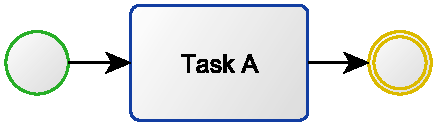
\includegraphics[width=0.5\linewidth]{bpmn2}
    \caption{A simple BPMN2 model.}
    \label{fig:bpmn2}
\end{figure}

Let's say that Bob developed a simple BPMN2 model in Fig. \ref{fig:bpmn2}. In common practice, if the model is persisted in state-based format, 
the persistence produces an XMI file (simplified) as in List. \ref{lst:bpmn2_xmi}. This type of persistence only preserves the eventual state of the model,  
loosing the detailed information of changes executed by Bob to construct the model. In contrary, 
if we record all the changes made by Bob and persist them into a CBP file, we can obtain a list of change events in List. \ref{lst:bpmn2_cbp}.
In this paper, the CBP file is pseudo-formatted to improve readability. In the real-world, the file is persisted in an XML-like format.
Replaying these recorded changes will produce a model with the same eventual state as in Fig. \ref{fig:bpmn2} and List. \ref{lst:bpmn2_xmi}.

\vspace{-15pt}
\begin{lstlisting}[style=eol,numbersep=1pt,caption={A BPMN2 model in Fig. \ref{fig:bpmn2} persisted in simplified XMI.},label=lst:bpmn2_xmi]
<process id="e1" name="Default Process">
 <startEvent id="e2">
   <outgoing>e6</outgoing>
 </startEvent>
 <endEvent id="e4">
   <incoming>e7</incoming>
 </endEvent>
 <task id="e5" name="Task A">
   <incoming>e6</incoming>
   <outgoing>e7</outgoing>
 </task>
 <sequenceFlow id="e6" sourceRef="e2" targetRef="e5"/>
 <sequenceFlow id="e7" sourceRef="e5" targetRef="e4"/>
</process>
\end{lstlisting}

From the list, we can know the sequence of changes made by Bob to construct the model. We can also identify that Bob made invalid changes 
that connect SequenceFlow \texttt{e3} from EndEvent \texttt{e4} to StartEvent \texttt{e2} 
(no SequenceFlow is allowed to come out from an EndEvent or enter a StartEvent) which he deleted later in the following changes. 
Such phenomenon might not be identified if we persists the model in state-based format. 

\vspace{-15pt}
\begin{lstlisting}[style=eol,numbersep=5pt,caption={The pseudo-formatted CBP of the model in Fig. \ref{fig:bpmn2}.},label=lst:bpmn2_cbp]
create e1 type Process
set e1.name to "Process 1"
create e2 type StartEvent
add e2 to e1.flowElements at 0
create e3 type SequenceFlow
set e3.name from to "Sequence Flow 1"
add e3 to e1.flowElements at 1
create e4 type EndEvent
add e4 to e1.flowElements at 0
add e3 to e2.incoming at 0
add e3 to e4.outgoing at 0
add e1 to resource at 0
remove e3 from e2.outgoing at 0 composite c1
remove e3 from e4.incoming at 0 composite c1
unset e3.name from "Sequence Flow 1" to null composite c1
remove e3 from e1.flowElements at 1 composite c1
delete e3 type SequenceFlow composite c1
create e5 type Task
set e5.name from to "Task 1"
add e5 to e1.flowElements at 2
create e6 type SequenceFlow
add e6 to e2.outgoing at 0
add e6 to e5.incoming at 0
add e6 to e1.flowElements at 3
create e7 type SequenceFlow
add e7 to e5.outgoing at 0
add e7 to e4.incoming at 0
add e7 to e1.flowElements at 4
set e5.name to "Task A"
\end{lstlisting}

While persisting all these changes is perceived too excessive as it requires more storage space \cite{DBLP:conf/models/YohannisRPK18}, 
in some conditions, it is desirable especially when we want to perform model analytics, 
such as understanding model evolution, identifying patterns, etc. \cite{DBLP:conf/models/YohannisKP17}. 
Moreover, CBP can also bring benefit to speed up model comparison \cite{yohannis2018efficient}.

Trying to understand changes executed by Bob in List. \ref{lst:bpmn2_cbp} may requires extra cognitive effort 
as one who tries to comprehend it needs to build a mental model and emulate the changes in his/her mind.
One solution to support users dealing with the cognitive effort is by providing an interactive visualisation tool.
With the tool, they can use it to replay the model construction and observe what kind of changes have been made by Bob.

\section{Visualising Model Construction}
\label{sec:visualising_model_construction}
We have built the CBP-Player, 
a simple prototype\footnote{Project and demo can be found at \url{https://github.com/alfa-ryano/CBP-Player} and \url{https://alfa-ryano.github.io/visualization.html}},
that visualise the construction of a model. The prototype can replay a CBP file in the form of animated graphical models.
It is a JavaScript application and uses mxGraph diagramming library \cite{mxgraph2019mxgraph} for displaying the graphical models. 

\subsection{Process}
\label{sec:process}
Fig. \ref{fig:process} shows the process of the CBP-Player in drawing a model. 
The process consist of three phases: Loading, Building, and Drawing.  
In the Loading phase, the CBP-Player loads a CBP file as change events in memory. 
It also load a predifined metamodel of the model represented in the CBP file. 
The metamodel defines the model that will be constructed by the Building phase.

\begin{figure}[h]
    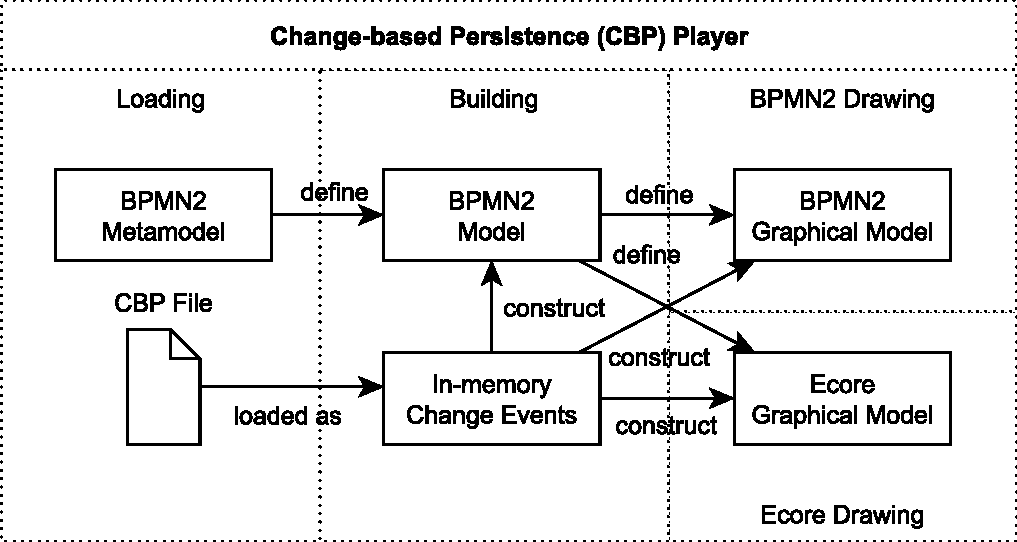
\includegraphics[width=\linewidth]{process}
    \caption{The process to visualise model construction using change-based persistence.}
    \label{fig:process}
\end{figure}

The CBP-Player plays the loaded change events one-by-one emulating the construction of the model in the CBP file.
The model needs to be constructed since it is useful for calculating certain values 
that are required in drawing its graphical representation.
For example, the shifting of elements' indexes caused by the deletion of an element in a containment or 
obtaining the type of a feature which is not available in the CBP file. 

When executing a change event, besides constructing the abstract model, 
a graphical model is also constructed. We can have more than one model drawer. 
In Fig. \ref{fig:process}, we have two drawings 
which allows to view a model construction in two perspectives: Ecore and BPMN2.

\subsection{Implementation}
\label{sec:implementation}
Fig. \ref{fig:class_diagram} depicts the simplified class diagram 
of the implementation of the CBP-Player. The main class \texttt{CBP-Player} has methods \texttt{load},
\texttt{play}, and \texttt{stop} to load and control the play of a CBP file.

\begin{figure}[h]
    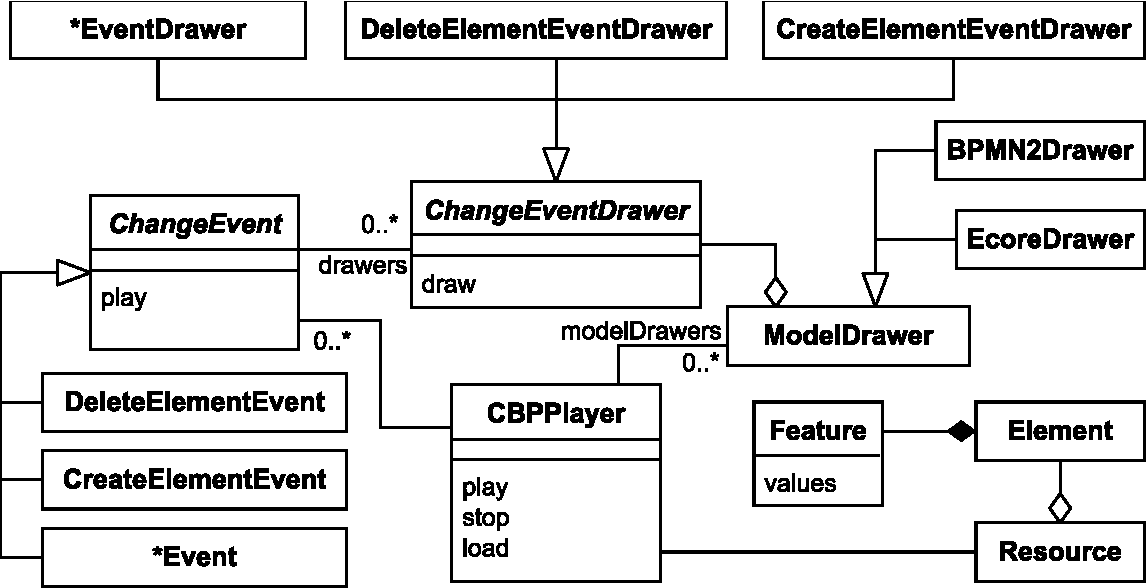
\includegraphics[width=\linewidth]{class_diagram}
    \caption{The simplified class diagram of the CBP-Player implementation.}
    \label{fig:class_diagram}
\end{figure}

When initialising, the \texttt{CBPPlayer} registers all kinds of \texttt{ModelDrawer} that are going to be used. 
In Fig. \ref{fig:class_diagram}, we use \texttt{EcoreDrawer} and \texttt{BPMN2Drawer} classes as examples for the model drawers. 
Both classes are derived from \texttt{ModelDrawer} class. This \texttt{ModelDrawer} class consists of 
different extension classes of the \texttt{ChangeEventDrawer} class. Each extension class determines
what kind of drawing operations should be executed on the graphical model if an instance of \texttt{ChangeEvent} is executed.
For example, when the play method of the \texttt{DeleteElementEventDrawer} class is executed,
it removes an element from the graphical model. The instance of this class is should be registered to
the its corresponding \texttt{ChangeEvent}, in this case, class \texttt{DeleteElementEvent}. 
If the instance of this \texttt{ChangeEvent} plays, it also executes the the \texttt{draw} method of 
the \texttt{ChangeEventDrawer} instances registered to it. Thus, if an element is deleted from an abstract model,
the corresponding element is also deleted in its graphical model. 

While executing the load method, a CBP file is loaded into memory as \texttt{changeEvents}, 
a list of \texttt{ChangeEvent}, and corresponding \texttt{ChangeEventDrawer} is registered to each change event. 
When \texttt{CBP-Player} plays this \texttt{changeEvents}, it iterates throughout the list and executes  
the \texttt{play} method of each change event emulating the construction of a model. 
After executing each \texttt{play} method, the \texttt{draw} method of 
the corresponding, registered \texttt{ChangeEventDrawer} is also executed to draw the model's graphic.
Classes \texttt{Resource}, \texttt{Element}, and \texttt{Feature} are used as internal data structures 
for constructing the abstract model.

\subsection{Application}
\label{sec:application}
To obtain the CBP file in List. \ref{lst:bpmn2_cbp}, firstly, we modify
the Eclipse BPMN2 modeler project \cite{eclipse2019bpmn2}. We add \texttt{ChangeEventAdapter} \cite{epsilonlabs2019changeeventadapter}
of the Epsilon CBP \cite{DBLP:conf/models/YohannisKP17}  to the \texttt{Bpmn2Resource}'s \texttt{eAdapters}
in the Eclipse BPMN2 modeler. Therefore, the adapater can capture every change made to a model on top of the modeller.
We create the model in Fig. \ref{fig:bpmn2} by following the course of changes in List. \ref{lst:bpmn2_cbp}.
We then save the model producing XMI and CBP files representative to the ones 
in Listings \ref{lst:bpmn2_xmi} and \ref{lst:bpmn2_cbp}. 
 
We have built a simple application in which we employ the CBP-Player. 
The application can visualise the construction of a BPMN2 model in two perspectives: Ecore and BPMN2. 
To demonstrate the application, we feed it with the produced CBP file. 
Fig. \ref{fig:prototype} shows a snapshot of the prototype at the time when edge \texttt{e3} 
is about to be removed (List. \ref{lst:bpmn2_cbp}, line 13) while replaying the CBP file.

\begin{figure}[h]
    \frame{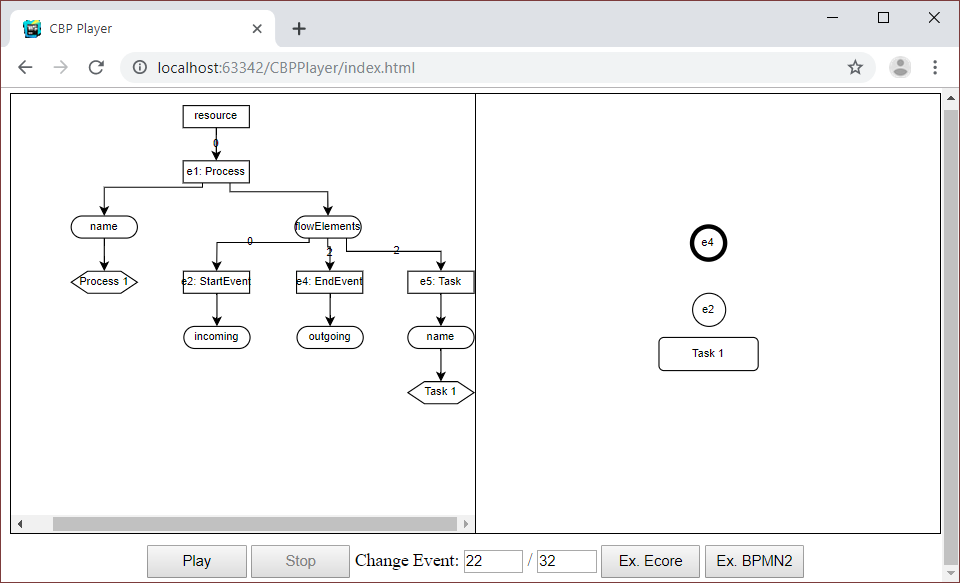
\includegraphics[width=\linewidth]{prototype}}
    \caption{A simple application that visualise the construction of the model in Fig. \ref{fig:bpmn2} in two perspective:
        Ecore and BPMN2.}
    \label{fig:prototype}
\end{figure}

\section{Evaluation}
\label{sec:evaluation}
We have not performed any performance evaluation in this work 
since performance is not the main goal of the current prototype.
To evaluate correctness, we have employed unit tests that exercises the features 
presented in this work. A more systematic evaluation is required in later iteration 
to evaluate the performance, usefulness, and usability of the CBP-Player.

\section{Related Work}
\label{sec:related_work}

\section{Conclusions and Future Work}
\label{sec:conclusions_and_future_work}
This paper has presented an extension to the work of change-based model persistence
that aims at providing a tool, the CBP-Player, to visualise model construction. 
The tool takes a CBP file as input and plays it in the form of graphical model
emulating the changes applied to the persisted model. 
The tool is designed to be extensible to any types of visualisation that aim
to exploit the information contained in CBP. The tool itself is still underdeveloped. 
Some features that are planned to be added are visualising model differencing
and conflict detection and model metrics 
(number of elements, features, etc.) throughout the evolution of a model.



\section*{Acknowledgment}
This work was partly supported by through a scholarship managed by \emph{Lembaga Pengelola Dana Pendidikan Indonesia} (Indonesia Endowment Fund for Education).

%\section*{References}
\bibliographystyle{IEEETran}
\bibliography{references}

\end{document}
